\documentclass[11pt,a4paper,openany,leqno]{article}

\textwidth=160mm \textheight=260mm \hoffset=-18mm \voffset=-30mm
\setcounter{page}{1}
			\usepackage[magyar]{babel}
			\usepackage[utf8]{inputenc}
			\usepackage[T1]{fontenc}
			\usepackage{indentfirst}
			\usepackage{amsmath,esint}
			\usepackage{amssymb}
%			\usepackage{eufrak}
			\usepackage{psfrag}
			\usepackage{tabularx}
			\usepackage{graphicx}
			\usepackage{wrapfig}	
			\usepackage{hyperref}
			\usepackage{multicol}	
									
			\frenchspacing
			\allowhyphens

\tolerance=2000
\hbadness=2000
\vbadness=10000
\overfullrule=0pt




\begin{document}
\section{Biot-Savart törvény}
\subsection{Kovács-Párkányi Fizikai Példatár II. / 441. feladat}


Az ábrán látható zárt vezetőben $I$ erősségű áram folyik. Határozzuk meg a mágneses térerősséget a szimmetria-középpontban!
\begin{figure}[h!]
\centering
  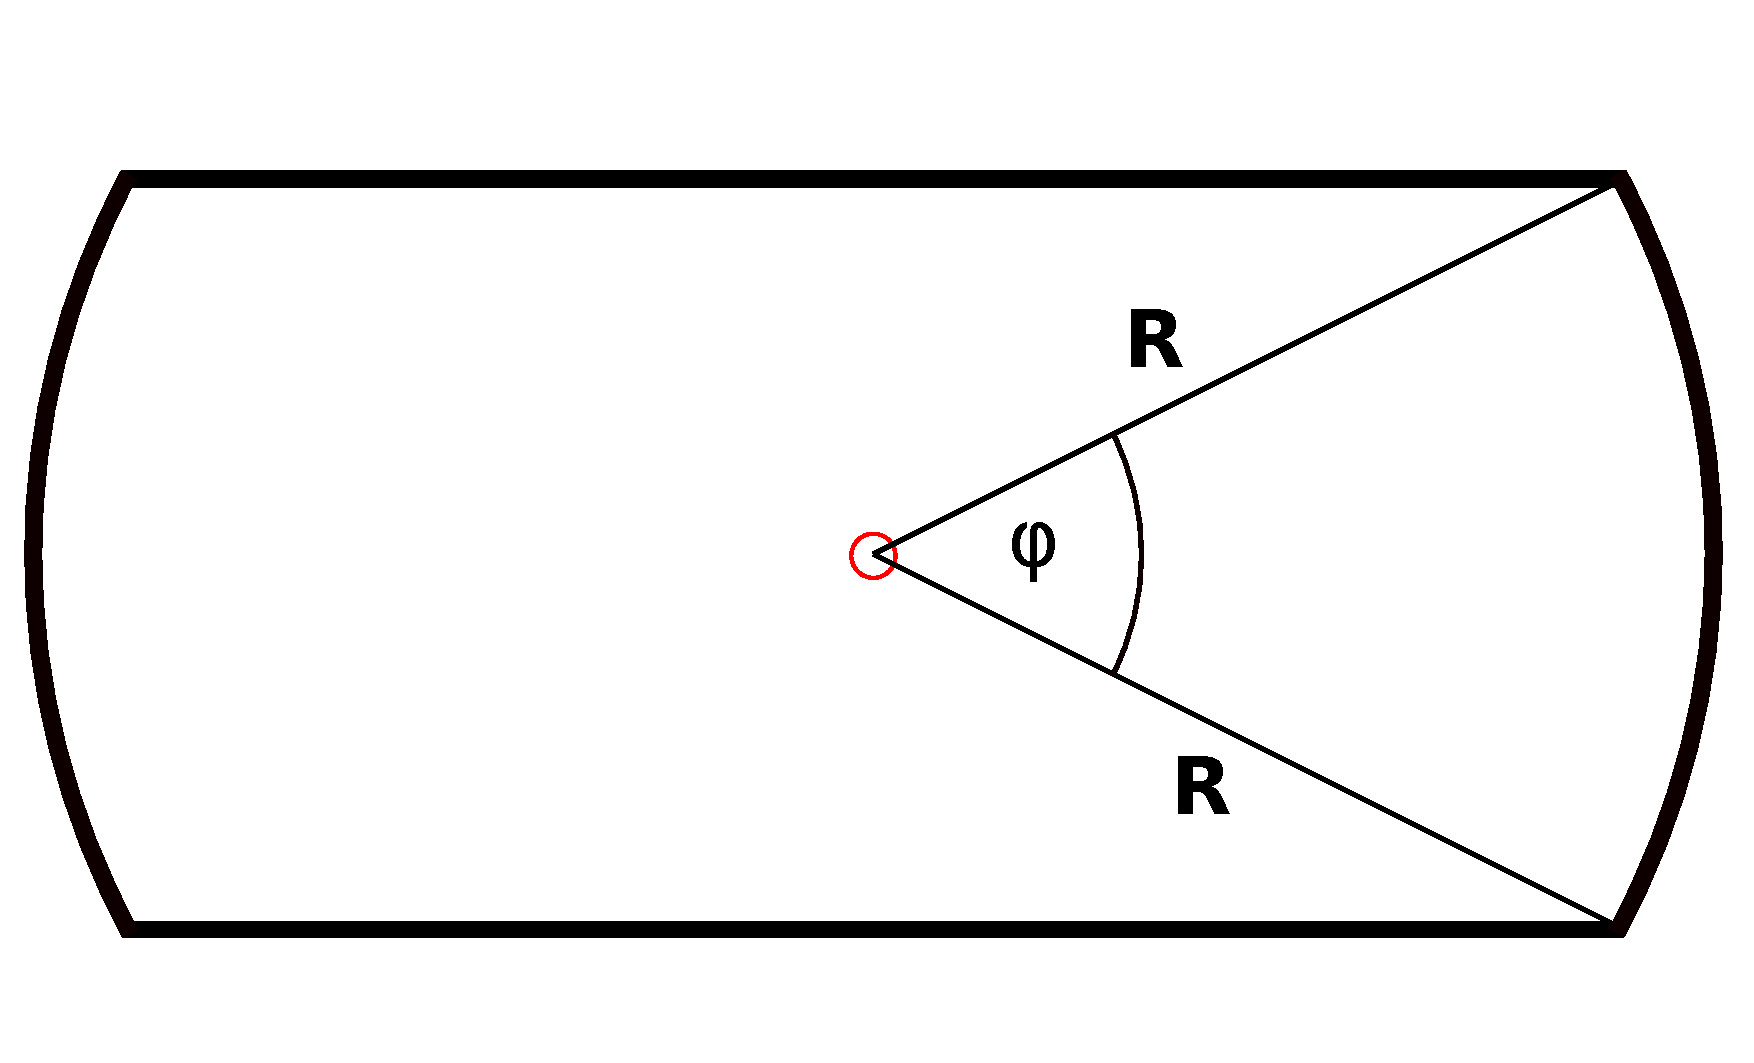
\includegraphics[width=120mm,scale=0.5]{abra.pdf}
  \caption{A vezető alakja}
  \label{}
\end{figure} \\ \indent
\indent

\begin{flushright} {Feladatot kidolgozta: {\it Z2R8XS}} \end{flushright}

\vspace{0.5cm}

\textbf{Megoldás}

Legyen koordinátarendszer origója a piros kör középpontja - itt határozandó meg a mágneses térerősség. Legyen a rendszer az $(x,y)$ síkban. A vezető alakja jellemezhető egy $G$ görbével. A Biot-Savart törvény értelmében
$$ \vec{B}(\vec{r}) = \frac{\mu_0}{4\pi}\int_{G} \frac{I \vec{r} \times d\vec{r}}{r^3} $$
\indent
Az áramerősség a görbe mentén konstans $I$ értéket vesz fel, a görbén kívül a tér minden pontjában $0$, így kiemelhető az integrál jel elé.
$$ \vec{B}(\vec{r}) = \frac{\mu_0 I}{4\pi}\int_{G} \frac{\vec{r} \times d\vec{r}}{r^3} $$
\newpage
\indent
Paraméterezni kell a görbét és kiszámolni az integrált. A görbe kényelmesen felszoltható négy részre az alábbi módon. Folyjon az áram pozitív irányba, azaz óramutató járásával ellentétben. A számok is árulkodnak arról, merre folyik az áram.
\begin{figure}[h!]
\centering
  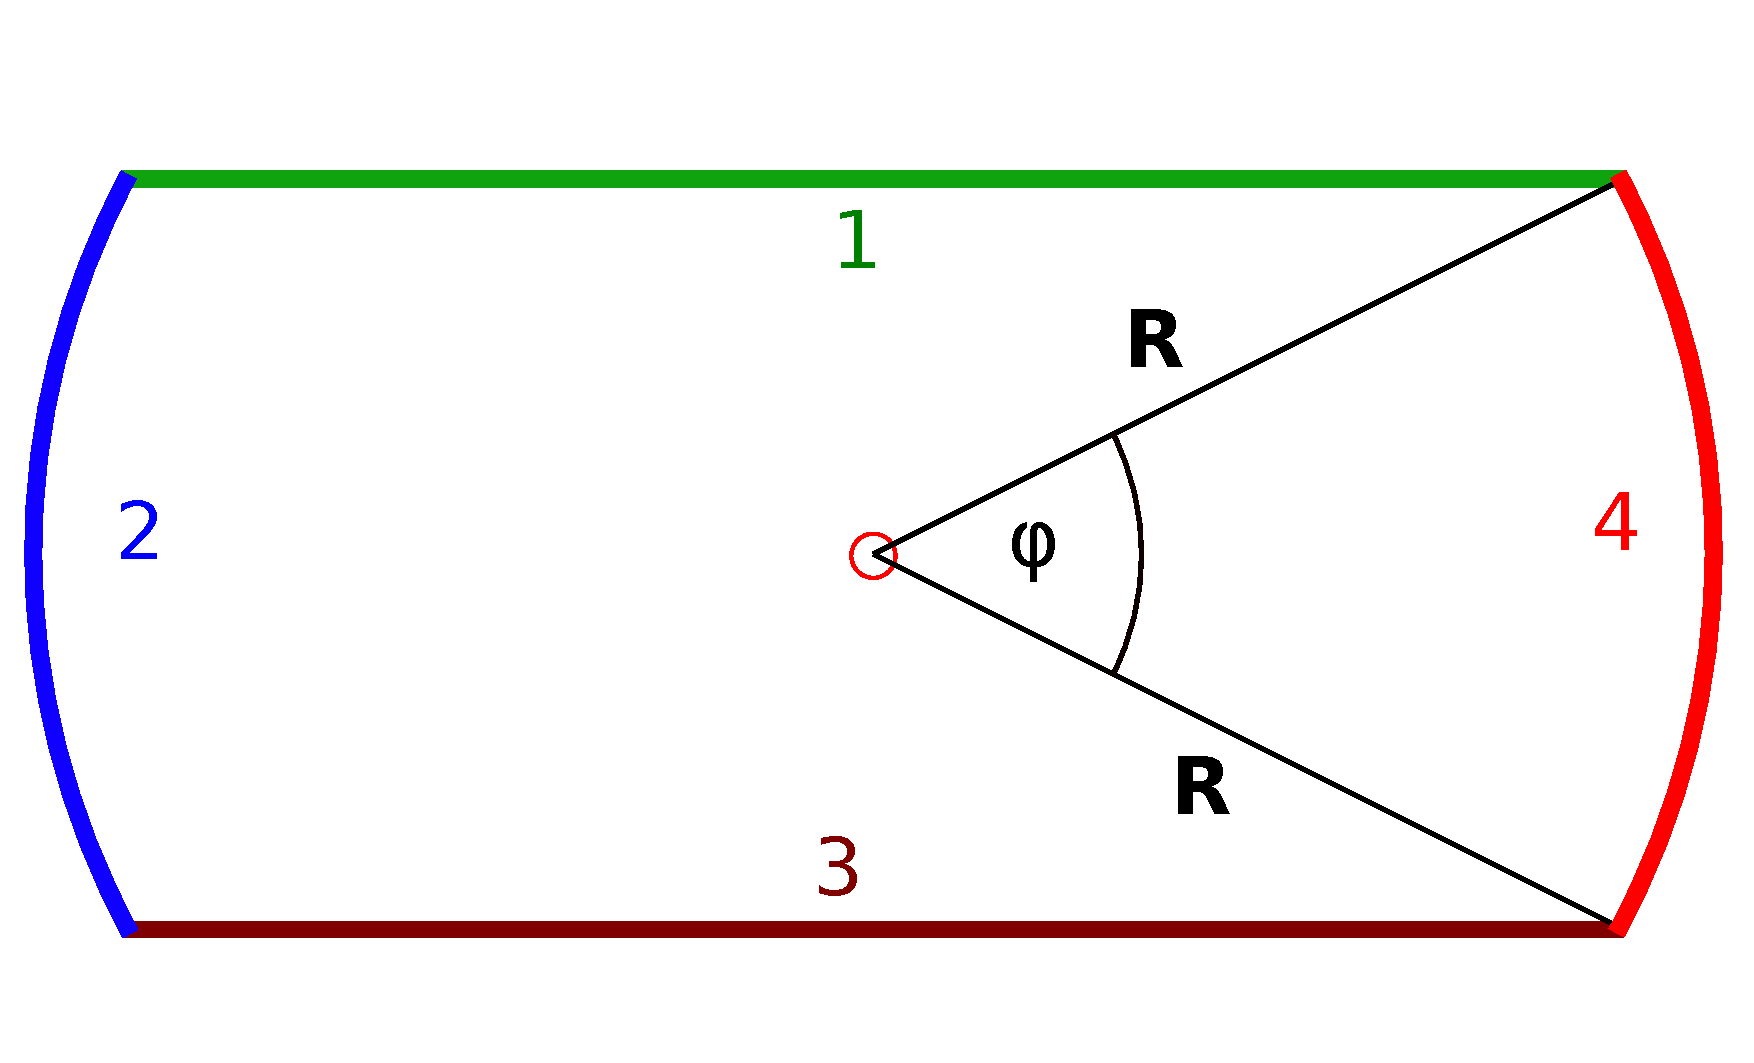
\includegraphics[width=120mm,scale=0.5]{felosztas.pdf}
  \caption{A görbe felosztása}
  \label{}
\end{figure} \\
\indent
Az $1.$ rész $x$-szel paraméterezhető:
$$ \vec{r} = \begin{pmatrix} x \\ R\cdot sin(\frac{\phi}{2}) \\ 0 \end{pmatrix} $$
$$ d\vec{r} = \begin{pmatrix} dx \\ 0 \\ 0 \end{pmatrix} $$
\indent
Azaz
$$ \vec{r} \times d\vec{r} = \begin{pmatrix} 0 \\ 0 \\ - R\cdot sin(\frac{\phi}{2}) \end{pmatrix} dx $$
$$ \vec{B}_1(\vec{r}(x)) = \frac{\mu_0 I}{4\pi}\int_{R cos(\frac{\phi}{2})}^{-Rcos(\frac{\phi}{2})} \frac{1}{(x^2 + R^2 \cdot sin^2 (\frac{\phi}{2}))^{3/2}}\cdot \begin{pmatrix} 0 \\ 0 \\ - R\cdot sin(\frac{\phi}{2}) \end{pmatrix} dx $$
\indent
Megfordíthatók az integrációs határok egy előjelváltás fejében.
$$ \vec{B}_1(x) = \frac{\mu_0 I R sin(\frac{\phi}{2})}{4\pi}\int_{-R cos(\frac{\phi}{2})}^{Rcos(\frac{\phi}{2})} \frac{1}{(x^2 + R^2 \cdot sin^2 (\frac{\phi}{2}))^{3/2}}\cdot \begin{pmatrix} 0 \\ 0 \\ 1 \end{pmatrix} dx $$
\indent
Foglalkozzunk az integrálandó vektor harmadik komponensével, oldjuk meg először határozatlan integrállal - hogy ne kelljen átírni a határokat.
$$ F(x) = \int \frac{1}{(x^2 + R^2 \cdot sin^2 (\frac{\phi}{2}))^{3/2}}\cdot dx $$
\indent
Legyen $ c^2 = R^2 \cdot sin^2 (\frac{\phi}{2}) $
$$ F(x) = \int \frac{1}{(x^2 + c^2)^{3/2}}\cdot dx $$
$$ F(x) = \frac{1}{c^3}\int \frac{1}{((\frac{x}{c})^2 + 1)^{3/2}}\cdot dx $$
\indent
Helyettsesítsük $tg(u) = \frac{x}{c}$-vel. Így $\frac{c\cdot du}{cos^2(u)} = dx $
$$ F(u) = \frac{1}{c^3}\int \frac{1}{(tg(u)^2 + 1)^{3/2}}\cdot \frac{c\cdot du}{cos^2(u)} $$
$$ F(u) = \frac{1}{c^2}\int \frac{1}{(tg(u)^2 + 1)^{3/2}}\cdot \frac{du}{ cos^2(u)} $$
$$ F(u) = \frac{1}{c^2}\int \frac{1}{(\frac{sin^2(u)}{cos^2(u)} + 1)^{3/2}}\cdot \frac{du}{cos^2(u)} $$
$$ F(u) = \frac{1}{c^2}\int \frac{1}{\frac{1}{cos^2(u)^{3/2}}}\cdot \frac{du}{cos^2(u)} $$
$$ F(u) = \frac{1}{c^2}\int cos(u) du $$
$$ F(u) = \frac{1}{c^2} sin(u) $$
$$ F(x) = \frac{1}{c^2} sin(arctg(\frac{x}{c})) $$
\indent
Ha $x$ és $c$ egy derékszögű háromszög befogói lennének, arányuk arkusz-tangense megandá az $c$ hosszúságú (szöggel szomszédos) befogó és a $\sqrt{x^2 + c^2}$ hosszúságú átfogó által bezárt szöget. Ennek a szögnek a szinusza megadja az $x$ hosszúságú (szöggel szemköztes) befogó és az átfogó arányát. Így
$$ F(x) = \frac{1}{R^2 \cdot sin^2(\frac{\phi}{2})} \frac{x}{\sqrt{x^2 + R^2 \cdot sin^2(\frac{\phi}{2})}} $$
\indent
Az itt megkapott $F(x)$ csak a primitív függvény. A határozott integrál értékét a határok segítségével kell kiszámolni. Legyen az integrál értéke $T$.
$$ T = [{\frac{1}{R^2 \cdot sin^2(\frac{\phi}{2})} \frac{x}{\sqrt{x^2 + R^2 \cdot sin^2(\frac{\phi}{2})}}}]_{-R\cdot cos(\frac{\phi}{2})}^{R \cdot cos(\frac{\phi}{2})} $$
$$T = \frac{1}{R^2 \cdot sin^2(\frac{\phi}{2})} \frac{R \cdot cos(\frac{\phi}{2})}{\sqrt{R^2 \cdot cos^2(\frac{\phi}{2}) + R^2 \cdot sin^2(\frac{\phi}{2})}} - \frac{1}{R^2 \cdot sin^2(\frac{\phi}{2})} \frac{- R \cdot cos(\frac{\phi}{2})}{\sqrt{R^2 \cdot cos^2(\frac{\phi}{2}) + R^2 \cdot sin^2(\frac{\phi}{2})}}$$
$$ T = \frac{2R cos(\frac{\phi}{2})}{R^2 \cdot sin^2(\frac{\phi}{2})}\cdot \frac{1}{\sqrt{R^2}} $$
$$ T = \frac{2 cos(\frac{\phi}{2})}{R^2 \cdot sin^2(\frac{\phi}{2})} $$
\indent Tehát
$$ \vec{B}_1 = \frac{\mu_0 I}{4\pi} \cdot \frac{2 cos(\frac{\phi}{2})}{R^2 \cdot sin^2(\frac{\phi}{2})} \begin{pmatrix} 0 \\ 0 \\ 1 \end{pmatrix}$$
$$ \vec{B}_1 = \frac{\mu_0 I}{2\pi} \cdot \frac{cos(\frac{\phi}{2})}{R^2 \cdot sin^2(\frac{\phi}{2})} \begin{pmatrix} 0 \\ 0 \\ 1 \end{pmatrix}$$
\indent
Belátható, hogy a $3.$ görbén integrálva egzaktul ugyenzt kapjuk, mivel ellentétes irányba folyik az áram, de az ellenkező irányban is integrálunk.\\
$$ \vec{B}_3 = \frac{\mu_0 I}{2\pi} \cdot \frac{cos(\frac{\phi}{2})}{R^2 \cdot sin^2(\frac{\phi}{2})} \begin{pmatrix} 0 \\ 0 \\ 1 \end{pmatrix}$$
\indent
A $2.$ és a $4.$ görbével hasonló lesz a helyzet, $\vec{B}_2 = \vec{B}_4$. Paraméterezzük a $4.$ görbét polárkoordináták segítségével. Mivel a $\phi$ név már foglalt, a szöget jelölő paraméter jele $\alpha$ lesz.
$$ \vec{r} = \begin{pmatrix} R\cdot cos(\alpha)  \\ R\cdot sin(\alpha) \\ 0 \end{pmatrix} $$
$$ d\vec{r} = \begin{pmatrix}  \\ -R\cdot sin(\alpha) \\ R\cdot cos(\alpha) \\ 0 \end{pmatrix} d\alpha $$
\indent
Láthatóan e két vektor mindig merőleges egymásra. Vektoriális szorzatuknak csak $z$ komponense van, valamint hossza a két vektor hosszának szorzata.
$$ \vec{r} \times d\vec{r} = \begin{pmatrix} 0 \\ 0 \\ R^2 \end{pmatrix} d\alpha $$
\indent Tehát
$$ \vec{B}_2 = \frac{\mu_0 I}{4\pi} \cdot \int_{-\phi/2}^{\phi/2} \frac{1}{R^3}\begin{pmatrix} 0 \\ 0 \\ R^2 \end{pmatrix} d\alpha $$

$$ \vec{B}_2 = \frac{\mu_0 I}{4\pi} \cdot \int_{-\phi/2}^{\phi/2} \frac{1}{R}\begin{pmatrix} 0 \\ 0 \\ 1 \end{pmatrix} d\alpha $$

$$ \vec{B}_2 = \frac{\mu_0 I}{4\pi} \cdot \frac{1}{R}\begin{pmatrix} 0 \\ 0 \\ \phi/2 - (-\phi/2) \end{pmatrix} $$

$$ \vec{B}_2 = \vec{B}_4 = \frac{\mu_0 I}{4\pi} \cdot \frac{\phi}{R}\begin{pmatrix} 0 \\ 0 \\ 1 \end{pmatrix} $$
\indent
Mindegyik huzalrész térerőssége pozitív $z$ irányba mutat - ez várható is volt a jobb kéz szabály miatt. Az egyes huzalrészek térerősségei összeadódnak.
$$ \vec{B} = \vec{B}_1 + \vec{B}_2 + \vec{B}_3 + \vec{B}_4 $$
$$ \vec{B} = \frac{2\mu_0 I}{2\pi} \cdot \frac{cos(\frac{\phi}{2})}{R^2 \cdot sin^2(\frac{\phi}{2})} \begin{pmatrix} 0 \\ 0 \\ 1 \end{pmatrix} + \frac{2\mu_0 I}{4\pi} \cdot \frac{\phi}{R}\begin{pmatrix} 0 \\ 0 \\ 1 \end{pmatrix} $$
\indent A rendszer által keltett mágneses tér a rendszer szimmetria-középpontjában
$$ \vec{B} = \frac{\mu_0 I}{2\pi} \cdot (2\frac{cos(\frac{\phi}{2})}{R^2 \cdot sin^2(\frac{\phi}{2})} + \frac{\phi}{R})\begin{pmatrix} 0 \\ 0 \\ 1 \end{pmatrix} $$
\indent
Ha ellenkező irányba folyna az áram, az egyenlőség jobb oldala megszorzódna $(-1)$-gyel.



\end{document}